\section*{Adversarial ML}

- We don't understand how NN models generalize and react to shifts in the distribution of data (i.e., distribution shifts)

- Classification problem: $(X,Y)\sim{\mathcal{D}},\;Y$ with range $\{-1,1\}$

- Standard risk: average zero-one loss over $X$: $R(f)=\mathbb{E}_{\mathcal{D}}\left[1_{f(X)\neq Y}\right]=\mathbb{P}_{\mathcal{D}}\left[f(X)\neq Y\right]$ i.e. minimise proba of wrong prediction.


- Adversarial risk: average zero-one loss over small, worst-case perturbations of $X$: $R_{\varepsilon}(f)={{{\mathbb{E}}}}_{\mathcal{D}}\left[\operatorname*{max}_{\hat{x},\|\hat{x}-X\|\leq\varepsilon}1_{f(\hat{x})\neq Y}\right]$

\subsection*{Generating adversarial examples}

- Task: given an input $(x, y)$ and a model $f : \mathcal{X}\rightarrow \{-1,1\}$ find an input $\hat{x}$ s.t.: 
a) $\|{\hat{x}}-x\|\leq\varepsilon$ b) the model $f$ makes a mistake on it.

- Trivial case: x already missclassified $\rightarrow$ no action required

- General case: ${\mathrm{find~}}{\hat{x}}~\mathrm{such~that}{\mathrm{~at}}f({\hat{x}})\neq y\operatorname{and}{\big\vert\vert}{\hat{x}}-x\vert\vert\leq\varepsilon$ i.e. $\hat{x}\in B_{x}(\varepsilon)\cap\{x^{\prime}f(x^{\prime})=-\,y\}$

- Optimization problem with respect to the inputs

- Problem: optimizing the indicator function is difficult: 1) The indicator function $1$ is not continuous 2) The NN prediction $f$ outputs discrete class values $\{-1,1\}$

- Replace the difficult problem involving the indicator with a smooth problem $\operatorname*{max}_{\hat{x},\|\hat{x}-X\|\leq\varepsilon}1_{f(\hat{x})\neq Y} \rightarrow \operatorname*{max}_{\hat{x},\|\hat{x}-X\|\leq\varepsilon}\ell(yg(\hat{x}))$

\begin{wrapfigure}{r}{0.5\columnwidth} 
    \centering
    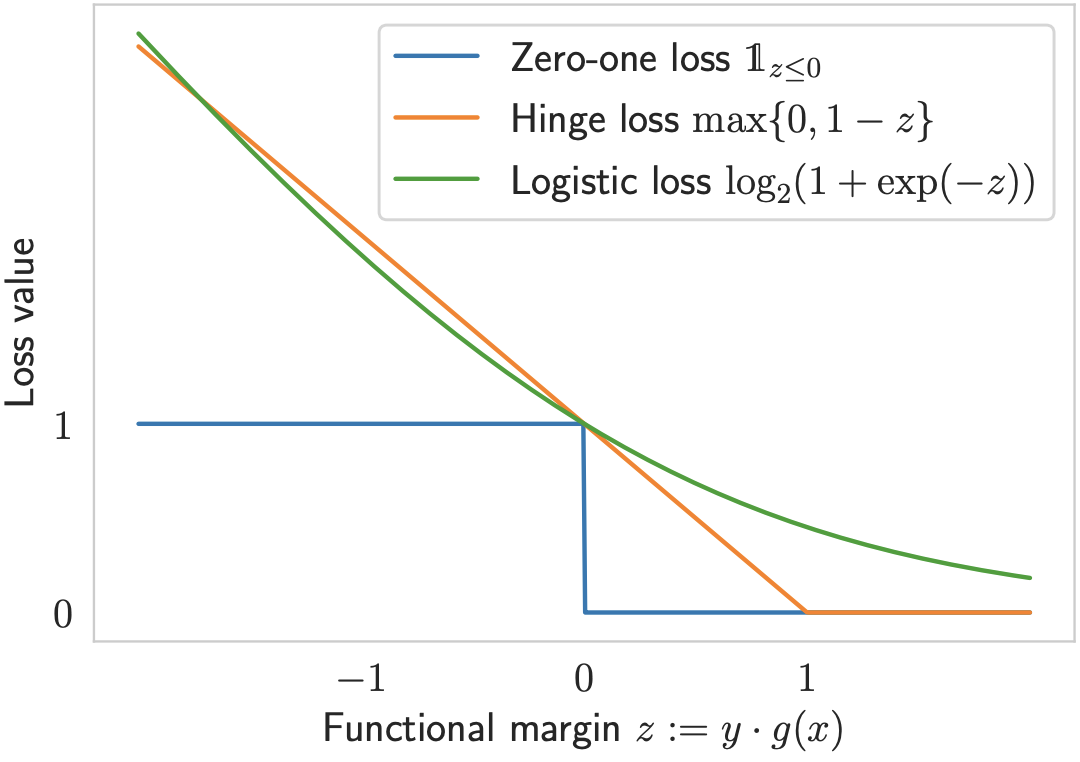
\includegraphics[width=0.5\columnwidth]{figures/classification_losses.png}
\end{wrapfigure}
- decreasing, margin-based (i.e., dependent on $y * g(x)$) classification losses

\subsection*{White-Box attacks}

- Solve $\operatorname*{max}_{\hat{x},\|\hat{x}-X\|\leq\varepsilon}\ell(yg(\hat{x}))$ knowing $g$

- $\nabla_{x}{\ell}(y g(x))=y\ell^{\prime}(y g(x))\,\nabla_{x}g(x)$, with $y\ell^{\prime}(y g(x)) \leq 0$ since classification losses are decreasing.

- Move in direction of $\propto-\,y\,\nabla_{x}g(x)$

- Interpretation $f(x)=\mathrm{{sign}}(g(x))$: If $y=1$ we want to decrease $g(x)$ and follow $-\nabla_{x}g(x)$. If $y=-1$ we want to decrease $g(x)$ and follow $\nabla_{x}g(x)$

- By using $\ell$ and not directly $yg(\hat{x})$ it will extend to multi-class classification and robust training.

- linearize the loss $\tilde{\ell}(x):={\ell}(y g(x))$

$\operatorname*{max}_{\|{\hat{x}}-x\|\leq\varepsilon}{\tilde{\ell}}(x)\\\approx\operatorname*{max}_{\|{\hat{x}}-x\|\leq\varepsilon}{\tilde{\ell}}(x)+\nabla_{x}{\tilde{\ell}}(x)^{T}({\hat{x}}-x) \\={\tilde{\ell}}(x)+\operatorname*{max}_{\|{\hat{x}}-x\|\leq\varepsilon}{\nabla}_{x}{\tilde{\ell}}(x)^{T}({\hat{x}}-x) \\={\tilde{\ell}}(x)+\operatorname*{max}_{\|\delta\|\leq\varepsilon}{\nabla}_{x}{\tilde{\ell}}(x)^{T}{\delta}$

- We need to maximize the inner product under a norm constraint, i.e. find the optimal local update

- This is a simple problem for which we can get a closed-form solution depending on the norm used to measure the perturbation size $||\delta||$

\subsubsection*{One-step attack}

- Solution for the $\ell_2$ norm:

$\delta_{2}^{\star}=\varepsilon\cdot\frac{\nabla_{x}\tilde{\ell}(x)}{||\nabla_{x}\tilde{\ell}(x)||_{2}}=-\;\varepsilon y*\frac{\nabla_{x}g(x)}{||\nabla_{x}g(x)||_{2}} \Rightarrow \\ \hat{x}=x-\varepsilon y\cdot\frac{\nabla_{x}g(x)}{\|\nabla_{x}g(x)\|_{2}}$

- Solution for the $\ell_{\infty}$ norm called \textbf{Fast Gradient Sign Method}:

$\delta_{\infty}^{\star}=\varepsilon\cdot\mathrm{sign}(\nabla_{x}\tilde{\ell}(x))=-\,\varepsilon y\cdot\mathrm{sign}(\nabla_{x}g(x)) \Rightarrow \\ {\hat{x}}=x-\varepsilon y\cdot\operatorname{sign}(\nabla_{x}g(x))$

\subsubsection*{Multi-step attack}


- These updates can be done iteratively and combined with a projection $\Pi$ on the feasible set (i.e., balls $\ell_2$ / $\ell_\infty$ here)

- Projected Gradient Descent (PGD attack)

- $\ell_2$ norm:

$\delta^{t+1}=\Pi_{B_{2}(e)} [\delta^{t}+\alpha\cdot\frac{\nabla\tilde{\ell}(x+\delta^{t})}{\|\nabla\tilde{\ell}(x+\delta^{t})\|_{2}}]$

$\Pi_{B_{2}(\varepsilon)}(\delta)=\left\{\begin{array}{l l}{\varepsilon\cdot\delta/\|\delta\|_{2},\quad{\mathrm{if~}}\|\delta\|_{2}\geq\varepsilon}\\ {\delta \mathrm{~otherwise}}\end{array}\right.$

- $\ell_\infty$ norm:

$\delta^{t+1}=\Pi_{B_{\infty}(\varepsilon)}\left[\delta^{t}+\alpha\cdot\mathrm{sign}(\nabla\tilde{\ell}(x+\delta^{t}))\right],$

$\Pi_{B_{\infty}(\varepsilon)}(\delta)_i=\left\{\begin{array}{l l}{\varepsilon\cdot\mathrm{sign}(\delta_{i}),\ \ \ \mathrm{if}\ |\delta_{i}|\geq\varepsilon}\\ {\delta_i \mathrm{~otherwise}}\end{array}\right.$

- the gradients are computed by backprop w.r.t. inputs, not parameters!

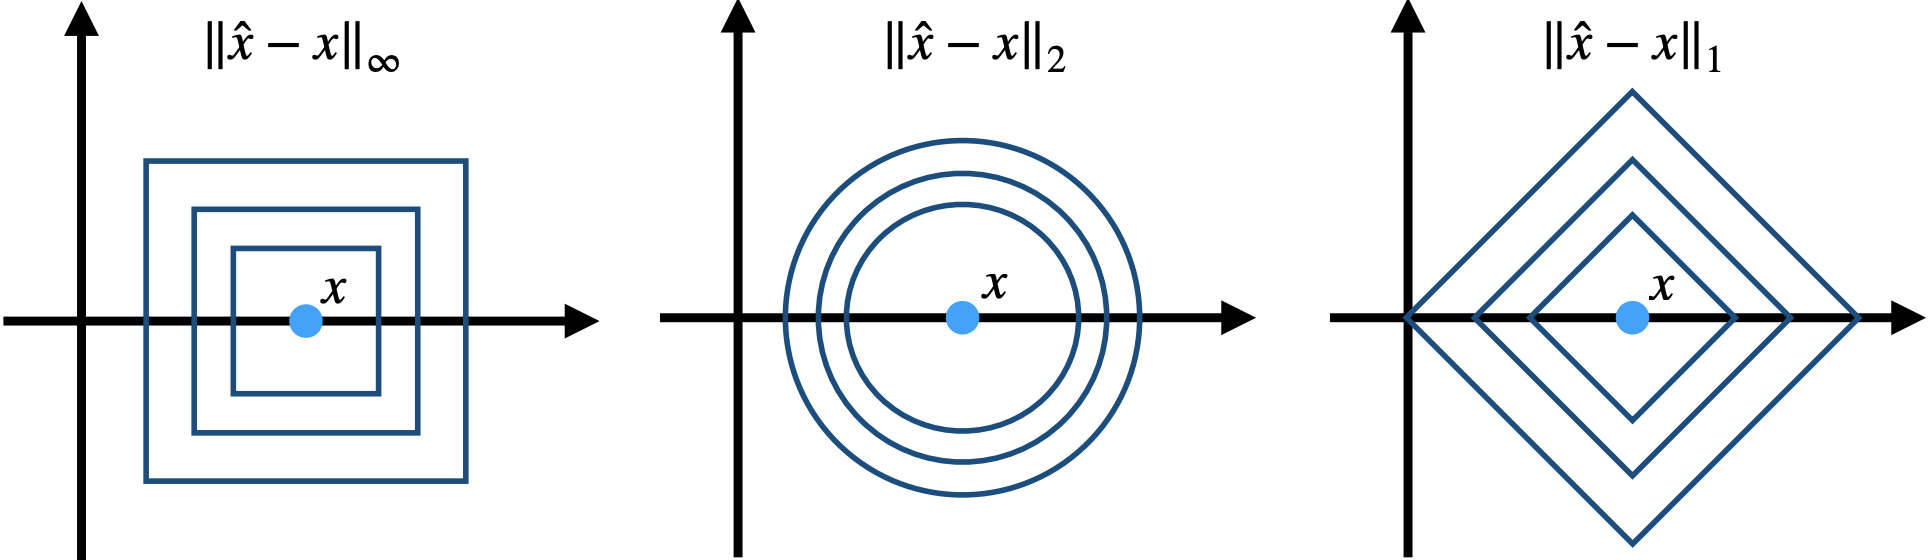
\includegraphics[width=\columnwidth]{figures/lp_norms.png}

\subsection*{Black-box attacks}

- We don't know $g(x)$

- Obtaining a surrogate model can be costly and there is no guarantee of success

- Query-based methods often require a lot of queries (10k-100k), easy to restrict access for the attacker!

\subsubsection*{Query-based gradient estimation}

- Score-based: we can query the continuous model scores $g(x)\in \mathbb{R}$. We can approximate the gradient by using the finite difference formula:

$\nabla_{x}g(x)\approx\sum_{i=1}^{d}\frac{g(x+\alpha e_{i})-g(x)}{\alpha}e_{i}$

- Decision-based: we can query only the predicted class $f(x) \in \{-1,1\}$, similar techniques can be adapted for the decision-based case.

\subsubsection*{Transfer Attacks}

- Train a similar surrogate model ${\hat{f}}\approx f$ on similar data

- Model stealing (query $f$ given some unlabeled inputs $\{x_{n},f(x_{n})\}_{n=1}^{N}$) can facilitate transfer attacks.


\subsection*{Adversarial training}

- Adversarial training: the goal is to minimize the adversarial risk:

$\operatorname*{min}_{\theta}R_{\varepsilon}(f_{\theta})=\mathbb{E}_{\mathcal{D}}\left[\operatorname*{max}_{\hat{x},\|\hat{x}-X\|\leq\varepsilon}1_{f(\hat{x})\neq Y}\right]$

- $\mathcal{D}$ unknown $\rightarrow$ approximate it with a sample average + classification loss is non-continuous $\rightarrow$ use a smooth loss $\Rightarrow$

$\operatorname*{min}_{\theta}{\frac{1}{N}}\sum_{n=1}^{N} \operatorname*{max}_{\hat{x}_{n},\|x_{n}-\hat{x}_{n}\|\leq\varepsilon}{\ell}(y_{n}g_{\theta}(\hat{x}_{n}))$

1) $\forall x_n\;, \hat{x}_{n}^{\star}\approx\arg\operatorname*{max}_{||x_{n}-\hat{x}_{n}|\leq\varepsilon}\ell(y_{n}g_{\theta}(\hat{x}_{n}))$

2) GD step w.r.t. $\theta$ using $\frac{1}{N}\sum_{n=1}^{N}\nabla_{\theta}{\ell}(y_{n}g_{\theta}({\hat{x}}_{n}^{\star}))$

\subsubsection*{Advantages}

- state-of-the-art approach for robust classification

- more interpretable gradients

- fully compatible with SGD

\subsubsection*{Disadvantages}

- Increased computational time: proportional to the number of PGD steps

- Robustness-accuracy tradeoff: using too large $\varepsilon$ leads to worse standard accuracy

\subsubsection*{Adversarial Example}
% \begin{wrapfigure}{r}{0.5\columnwidth} 
%     \centering
%     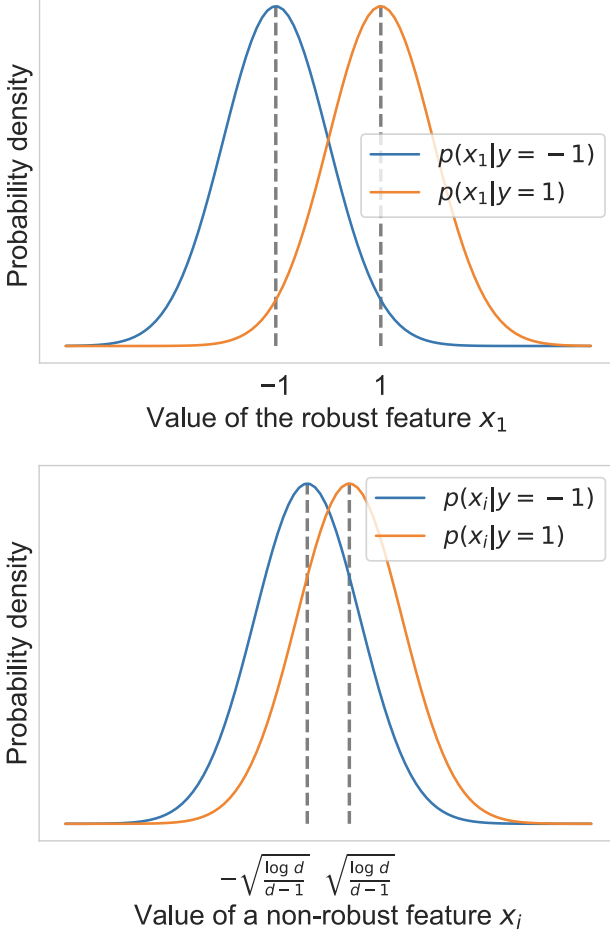
\includegraphics[width=0.5\columnwidth]{figures/adversarial_example.png}
% \end{wrapfigure}

$x\in\mathbb{R}^{d},y\sim{{Bernoulli}}(\{-1,1\}),Z_{i}\sim{\mathcal{N}}(0,1)$

- Robust features: $x_{1}=y+Z_{1}$

- Non-robust features: $x_{i}=y{\sqrt{\frac{\log d}{d-1}}}+Z_{i}, \; \forall i \in \{-1, 1\}$

- $d\to\infty \Rightarrow \ \uparrow$ adversarial risk and $\downarrow$ standard risk 

- using the robust feature $x_1$:

MLE: $\arg\operatorname*{max}_{\hat{y}\in\{\pm1\}}p(\hat{y}\;\vert\;x_{1})
=\\\operatorname*{arg}\operatorname*{max}_{{\hat{y}}\in\{\pm1\}}{\frac{p(x_{1}\mid{\hat{y}})p({\hat{y}})}{p(x_{1})}}
=\operatorname*{arg}\operatorname*{max}_{{\hat{y}}\in\{\pm1\}}{p(x_{1}\mid{\hat{y}})}$ 
assuming $p(y=1)=p(y=-1)$

- Standard Risk: $\int_{0}^{\infty}{\frac{1}{\sqrt{2\pi}}}e^{-0.5(x+1)^{2}}d x\approx0.16$ good but not perfect!

- using both robust and non-robust features:

MLE for all features $x_{i}=y a_{i}+Z_{i}$

$\arg\operatorname*{max}_{{\hat{y}}\in\{\pm1\}}p({\hat{y}}\mid x)$

$=\arg\operatorname*{max}_{{\hat{y}}\in\{\pm1\}}\prod_{i=1}^{d}p(x_{i}\mid{\hat{y}})$

$=\arg\operatorname*{max}_{{\hat{y}}\in\{\pm1\}}\sum_{i=1}^{d}\log p(x_{i}\mid{\hat{y}})$

$=\arg\operatorname*{max}_{{\hat{y}}\in\{\pm1\}}\sum_{i=1}^{d}\log \frac{1}{\sqrt{2\pi}}e^{-\frac{1}{2}(x_{i}-\hat{y}a_{i})^{2}}$

$=\arg\operatorname*{min}_{{\hat{y}}\in\{\pm1\}}\sum_{i=1}^{d}(x_{i}-\hat{y}a_{i})^{2}$

$=\arg\operatorname*{min}_{{\hat{y}}\in\{\pm1\}}\sum_{i=1}^{d}(x_{i}^{2}-2x_{i}\hat{y}a_{i}+\hat{y}^{2}a_{i}^{2})$

$=\arg\operatorname*{max}_{\hat{y}\in\{\pm1\}}{\hat{y}}\sum_{i=1}^{d}x_{i}a_{i}$

${\hat{y}}\sum_{i=1}^{d}x_{i}a_{i}=\hat{y}y(\sum_{i=1}^{d}a_{i}^{2})+\hat{y}\sum_{i=1}^{d}a_{i}Z_{i}=\hat{y}y(1+\log(d))+\hat{y}Z$ where $Z:=\textstyle\sum_{i=1}^{d}a_{i}Z_{i}\sim{\mathcal{N}}(0,1+\log d)$

Scaling by $1/(1+\log d)$ the MLE results in:

$y{\hat{y}}+{\hat{y}}Z\operatorname{with}Z\sim{\mathcal{N}}(0,1/(1+\log d))$

$d\rightarrow\infty,{\hat{y}}Z\rightarrow0 \Rightarrow$ standard risk $R(f) \rightarrow 0$ 

- using the non-robust features improves standard risk!

- Adversarial risk:

The adversary can use tiny $\ell_\infty$ perturbations:

$\varepsilon=2\sqrt{\frac{\log d}{d-1}}\,(\to0\,\mathrm{when})\,d\to\infty)$

${\hat{x}}_{1}=\left(1-2\sqrt{\frac{\log d}{d-1}}\right)y+Z_{1}$, almost unaffected

$\hat{x}_{i}=-\sqrt{\frac{\log d}{d-1}}y+Z_{i}$, completely flipped

$R_{\varepsilon}(f) \approx 1 \Rightarrow$ tradeoff between accuracy and robustness.
